\documentclass[tikz, border=10pt]{standalone}

\usetikzlibrary{arrows}

\begin{document}
	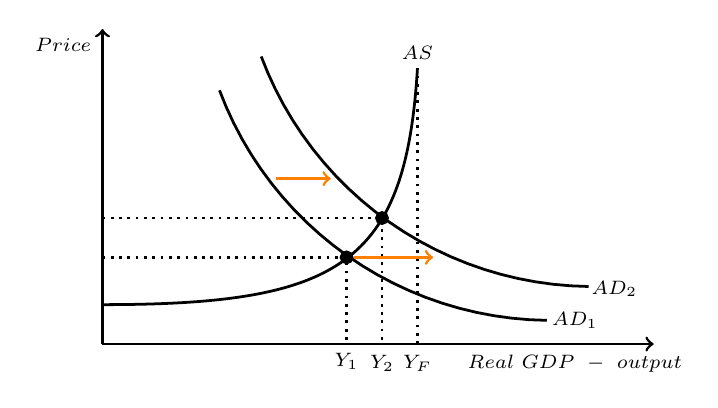
\begin{tikzpicture}[line width=1pt]
	
	\draw[->] (0, 0) -- (7, 0); % Горизонтальная линия
	\draw[->] (0, 0) -- (0, 4); % Вертикальная линия

	\draw (0, 0.5) .. controls (3, 0.5) and (3.85, 1) .. (4, 3.5); % Кривая AS
	
	\draw[fill=black] (3.1, 1.1) circle (2pt); 
	\draw[fill=black] (3.55, 1.6) circle (2pt);
	
	\draw [shift={(6.23, 5.23)}] plot[domain=3.5:4.7,variable=\t]({1*4.5*cos(\t r)+-0*4*sin(\t r)},{0*4*cos(\t r)+1*4.5*sin(\t r)});
	\draw [shift={(5.7, 4.8)}] plot[domain=3.5:4.7,variable=\t]({1*4.5*cos(\t r)+-0*4*sin(\t r)},{0*4*cos(\t r)+1*4.5*sin(\t r)});
	
	\draw[dotted] (0, 1.1) -- (3.1, 1.1) -- (3.1, 0);
	\draw[dotted] (0, 1.6) -- (3.55, 1.6) -- (3.55, 0);
	
	\draw[dotted] (4, 0) -- (4, 3.5);

	\draw[->, color=orange] (2.2, 2.1) -- (2.9, 2.1);
	\draw[->, color=orange] (3.2, 1.1) -- (4.2, 1.1);

	\begin{scriptsize}
		\draw (-0.5, 3.8) node {$Price$};
		\draw (6, -0.25) node {$Real~GDP~-~output$};
		
		\draw (3.1, -0.225) node {$Y_{1}$};
		
		\draw (3.55, -0.25) node {$Y_{2}$};
		\draw (4, -0.25) node {$Y_{F}$};
		
		\draw (4, 3.7) node {$AS$};
		\draw (6.5, 0.7) node {$AD_{2}$};
		\draw (6, 0.3) node {$AD_{1}$};
	\end{scriptsize}
	\end{tikzpicture}
\end{document}